\documentclass{report}
\usepackage[T1]{fontenc} % Fontes T1
\usepackage[utf8]{inputenc} % Input UTF8
\usepackage[backend=biber, style=ieee]{biblatex} % para usar bibliografia
\usepackage{csquotes}
\usepackage[portuguese]{babel} %Usar língua portuguesa
\usepackage{blindtext} % Gerar texto automaticamente
\usepackage[printonlyused]{acronym}
\usepackage{hyperref} % para autoref
\usepackage{graphicx}
\usepackage{placeins}
\bibliography{bibliografia}


\begin{document}
%%
% Definições
%
\def\titulo{Cliente de chat}
\def\data{21/04/2016}
\def\autores{Alexandre Lourenço, Ana Margarida Silva, Susana Dias}
\def\autorescontactos{(79894) alexandre.lourenco@ua.pt, (77752) margaridaocs@ua.pt, (80410) susanadias@ua.pt}
\def\versao{VERSAO 1.0}
\def\departamento{Departamento de Eletrónica, Telecomunicações e Informática}
\def\empresa{Universidade de Aveiro}
\def\logotipo{ua.pdf}
%
%%%%%% CAPA %%%%%%
%
\begin{titlepage}

\begin{center}
%
\vspace*{50mm}
%
{\Huge \titulo}\\ 
%
\vspace{10mm}
%
{\Large \empresa}\\
%
\vspace{10mm}
%
{\LARGE \autores}\\
%
\vspace{30mm}
%
\begin{figure}[h]
\center
\includegraphics{\logotipo}
\end{figure}
%
\vspace{30mm}
\end{center}
%
\begin{flushright}
\versao
\end{flushright}
\end{titlepage}

%%  Página de Título %%
\title{
{\Huge\textbf{\titulo}}\\
{\Large \departamento\\ \empresa}
}
%
\author{
\textbf{
    {\center \autores } \\
    {\center \autorescontactos} \\
}
}

\date{\data}

\maketitle

\pagenumbering{roman}

%%%%%% RESUMO %%%%%%
\begin{abstract}
Com este trabalho de aprofundamento desenvolvemos um cliente de chat em python, com recurso a sockets e json, que permite enviar e receber mensagens para os restantes utilizadores.
\end{abstract}

%%%%%% Agradecimentos %%%%%%
% Segundo glisc deveria aparecer após conclusão...\
%\renewcommand{\abstractname}{Agradecimentos}
%\begin{abstract}
%Eventuais agradecimentos.
%Comentar bloco caso não existam agradecimentos a fazer.
%\end{abstract}


\tableofcontents
% \listoftables     % descomentar se necessário
% \listoffigures    % descomentar se necessário


%%%%%%%%%%%%%%%%%%%%%%%%%%%%%%%
\clearpage
\pagenumbering{arabic}

%%%%%%%%%%%%%%%%%%%%%%%%%%%%%%%%
\chapter{Introdução}
\label{chap.introducao}

Cada vez mais a comunicação a longas distâncias é facilitada com recurso a transmissões de pacotes de dados pela internet entre utilizadores, e foi nessa perspectiva que este trabalho foi concebido, tendo como vista a criação de uma interface que permitisse connectar vários clientes a um servidor criando assim um chat em python que recorre a json para formatação das mensagens enviadas, posteriormente, em sockets.

\chapter{Arquitetura da aplicação}
\label{chap.arquitetura}

A ligação ao servidor LabiChat é feita pelo protocolo TCP/IP conectando-se ao endereço 37.247.48.69 pela porta 1863. O cliente é composto por três funções fora da main() que representam comandos que podem ser executados pelo utilizador.

\section{getOn()}
Converte o campo "to" e imprime no terminal todas as pessoas que se encontram online no momento.

\section{nickname()}
Altera o nickname do utilizador. Quando esta função é invocada, o campo "from" é substituído pela string inserida.

\section{message()}
Recebe duas strings (data0 e data1) e converte-as em json como mensagem e destinatário respetivamente. Se a mensagem for vazia, não será enviada.

\section{main()}
Gere tudo o que é enviado e recebido no socket. Após receber o nickname do utilizador, fica à espera de uma resposta do servidor ou de um pedido do cliente. O módulo select.select() é utilizado para que apenas receba mensagens quando não está uma mensagem a ser digitada, pois isso daria origem a uma quebra. \\
Ao digitar uma das opções, a respetiva função será executada, à exceção do caso do comando sair, em que o programa será terminado.
\chapter{Utilização do cliente}
\label{chap.util}
Para aceder ao chat terá de ser introduzido no terminal "python clientFinal2.py".\\

\section{Opções de Utilização:} \\
\\
sair - Para quando o utilizador quiser sair do programa \\
online - O cliente será informado de quem se encontra online \\
msg - Será possível para o cliente escolher o destinatário para quem deseja enviar a mensagem e escrever a mensagem \\
nome - será permitido ao cliente mudar de nome

%imagens dos resultados obtidos
\section{Exemplos}
\begin{figure}[!htp]
\centering
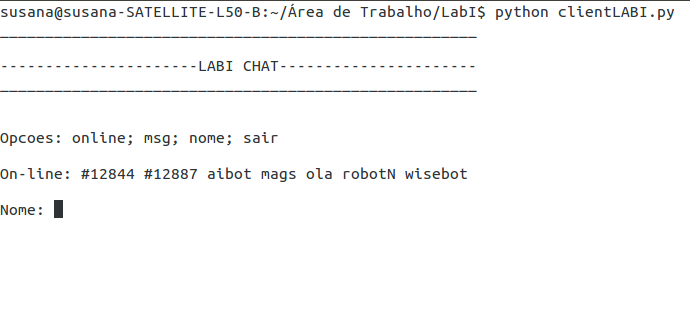
\includegraphics[scale=0.35]{inicio.png} 
\caption{Aceder à consola}
\end{figure}
 
\begin{figure}[!htp]
\centering
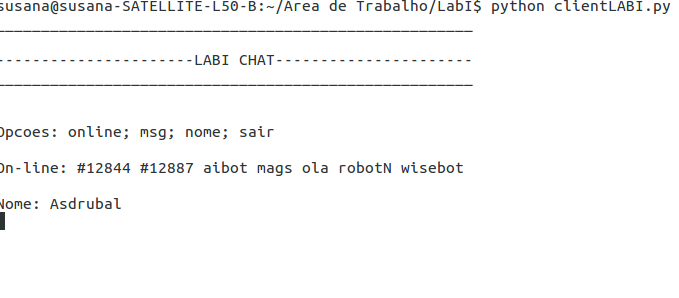
\includegraphics[scale=0.5]{nome.png} 
\caption{Nome de utilizador}
\end{figure}

\begin{figure}
\centering
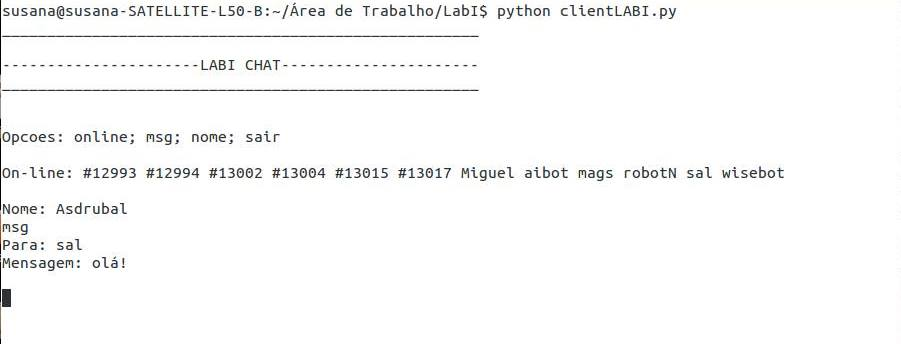
\includegraphics[scale=0.5]{msg.jpeg}
\caption{Envio de mensagem}
\end{figure}

\begin{figure}
\centering
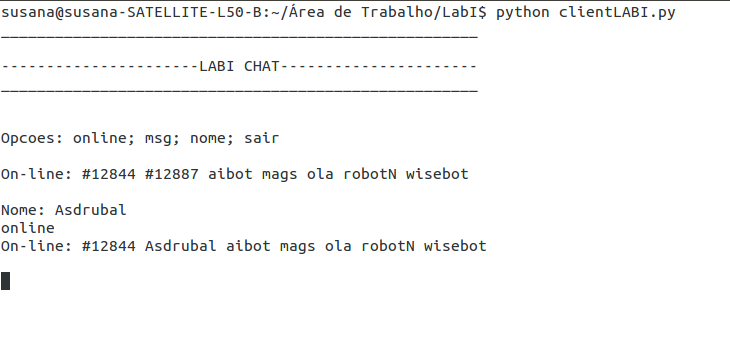
\includegraphics[scale=0.5]{online.png} 
\caption{Utilizadores online}
\end{figure}

\begin{figure}
\centering
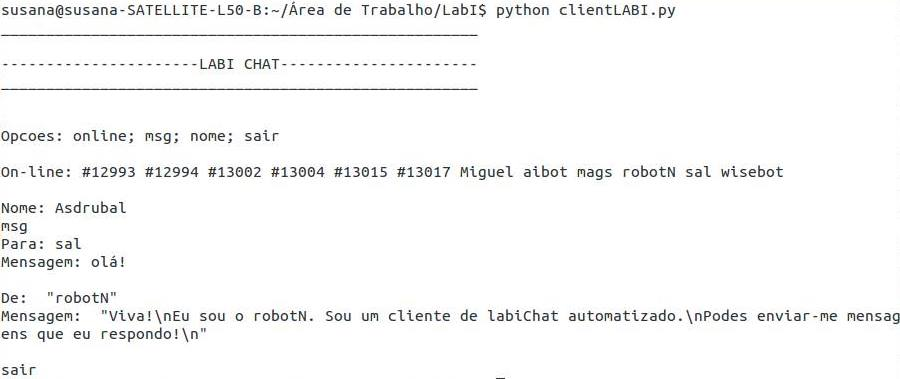
\includegraphics[scale=0.5]{sair.jpeg} 
\caption{Terminar chat}
\end{figure}


\chapter*{Contribuições dos autores}

\begin{itemize}
    \item Alexandre Lourenço (40\%)
    \item Ana Margarida Silva (30\%)
    \item Susana Dias (30\%)



\end{document}
